% Options for packages loaded elsewhere
\PassOptionsToPackage{unicode}{hyperref}
\PassOptionsToPackage{hyphens}{url}
%
\documentclass[
]{article}
\usepackage{lmodern}
\usepackage{amssymb,amsmath}
\usepackage{ifxetex,ifluatex}
\ifnum 0\ifxetex 1\fi\ifluatex 1\fi=0 % if pdftex
  \usepackage[T1]{fontenc}
  \usepackage[utf8]{inputenc}
  \usepackage{textcomp} % provide euro and other symbols
\else % if luatex or xetex
  \usepackage{unicode-math}
  \defaultfontfeatures{Scale=MatchLowercase}
  \defaultfontfeatures[\rmfamily]{Ligatures=TeX,Scale=1}
\fi
% Use upquote if available, for straight quotes in verbatim environments
\IfFileExists{upquote.sty}{\usepackage{upquote}}{}
\IfFileExists{microtype.sty}{% use microtype if available
  \usepackage[]{microtype}
  \UseMicrotypeSet[protrusion]{basicmath} % disable protrusion for tt fonts
}{}
\makeatletter
\@ifundefined{KOMAClassName}{% if non-KOMA class
  \IfFileExists{parskip.sty}{%
    \usepackage{parskip}
  }{% else
    \setlength{\parindent}{0pt}
    \setlength{\parskip}{6pt plus 2pt minus 1pt}}
}{% if KOMA class
  \KOMAoptions{parskip=half}}
\makeatother
\usepackage{xcolor}
\IfFileExists{xurl.sty}{\usepackage{xurl}}{} % add URL line breaks if available
\IfFileExists{bookmark.sty}{\usepackage{bookmark}}{\usepackage{hyperref}}
\hypersetup{
  pdftitle={How many researchers use `boilerplate' statistical analysis sections?},
  pdfauthor={Nicole White, Thiru Balasubramaniam, Richi Nayak, Adrian Barnett},
  hidelinks,
  pdfcreator={LaTeX via pandoc}}
\urlstyle{same} % disable monospaced font for URLs
\usepackage[margin=1in]{geometry}
\usepackage{graphicx,grffile}
\makeatletter
\def\maxwidth{\ifdim\Gin@nat@width>\linewidth\linewidth\else\Gin@nat@width\fi}
\def\maxheight{\ifdim\Gin@nat@height>\textheight\textheight\else\Gin@nat@height\fi}
\makeatother
% Scale images if necessary, so that they will not overflow the page
% margins by default, and it is still possible to overwrite the defaults
% using explicit options in \includegraphics[width, height, ...]{}
\setkeys{Gin}{width=\maxwidth,height=\maxheight,keepaspectratio}
% Set default figure placement to htbp
\makeatletter
\def\fps@figure{htbp}
\makeatother
\setlength{\emergencystretch}{3em} % prevent overfull lines
\providecommand{\tightlist}{%
  \setlength{\itemsep}{0pt}\setlength{\parskip}{0pt}}
\setcounter{secnumdepth}{-\maxdimen} % remove section numbering

\title{How many researchers use `boilerplate' statistical analysis sections?}
\usepackage{etoolbox}
\makeatletter
\providecommand{\subtitle}[1]{% add subtitle to \maketitle
  \apptocmd{\@title}{\par {\large #1 \par}}{}{}
}
\makeatother
\subtitle{An observational study of papers published in \emph{PLOS ONE}.}
\author{Nicole White, Thiru Balasubramaniam, Richi Nayak, Adrian Barnett}
\date{21/05/2020}

\begin{document}
\maketitle

An ideal statistical analysis will use appropriate methods to create
insights from the data and inform the research questions. Unfortunately
many current statistical analyses are far from ideal, with many
researchers using the wrong methods, misinterpreting the results, or
failing to adequately check their assumptions (Goodman
\protect\hyperlink{ref-Goodman2008}{2008}; Leek et al.
\protect\hyperlink{ref-Leek2017}{2017}). Some researchers take a
``mechanistic'' approach to statistics, copying the few methods they
know regardless of their appropriateness, and then going through the
motions of the analysis (Stark and Saltelli
\protect\hyperlink{ref-Stark2018}{2018}).

Many researchers lack adequate training in research methods, and
statistics is something they do with trepidation and even ignorance
(Altman \protect\hyperlink{ref-Altman1994}{1994}; King et al.
\protect\hyperlink{ref-King2019}{2019}). However, using the wrong
statistical methods can cause real harm (Altman
\protect\hyperlink{ref-Altman1994}{1994}) and bad statistical practices
are being to used abet weak science (Stark and Saltelli
\protect\hyperlink{ref-Stark2018}{2018}). Statistical mistakes are a key
source of waste in research and partly explain the current
reproducibility crisis in science (Allison et al.
\protect\hyperlink{ref-Allison2016}{2016}). Even when the correct
methods are used, many researchers fail to describe them adequately,
making it difficult to reproduce the results (Ernst and Albers
\protect\hyperlink{ref-Ernst2017}{2017}; Zhou and Skidmore
\protect\hyperlink{ref-Zhou2018}{2018}).

The International Committee of Medical Journal Editors recommend that
researchers should: ``Describe statistical methods with enough detail to
enable a knowledgeable reader with access to the original data to judge
its appropriateness for the study and to verify the reported results''
(ICJME \protect\hyperlink{ref-ICMJE2019}{2019}). Although the general
lack of statistical understanding from both authors and reviewers means
this recommendation may not be checked. A recent survey of editors found
that only 23\% of health and medical journals used expert statistical
review for all articles (Hardwicke and Goodman
\protect\hyperlink{ref-Hardwicke2020}{2020}), which was little different
from a survey from 22 years ago (Goodman, Altman, and George
\protect\hyperlink{ref-Goodman1998}{1998}).

Two statisticians on this paper (AB and NW) have heard researchers admit
that they sometimes copy-and-paste their statistical methods sections
from other papers, regardless of whether they are appropriate. The aim
of this paper is to use text-mining methods to estimate the extent that
researchers are using cut-and-paste or `boilerplate' statistical methods
sections. Use of these methods sections indicates that little thought
has gone into the statistical analysis.

\hypertarget{methods}{%
\section{Methods}\label{methods}}

\hypertarget{data-sources}{%
\subsection{Data sources}\label{data-sources}}

We used two openly available data sources to find statistical methods
sections.

\hypertarget{public-library-of-science-plos-one}{%
\subsubsection{Public Library of Science (PLOS
ONE)}\label{public-library-of-science-plos-one}}

\emph{PLOS ONE} is a large open access journal that publishes original
research across a wide range of scientific fields. Articles must be in
English. Article submissions are handled by an academic editor who
selects peer reviewers based on their self-nominated area(s) of
expertise. Submissions do not undergo formal statistical review.
Instead, reviewers are required to assess submissions against several
publication criteria, including whether: ``Experiments, statistics, and
other analyses are performed to a high technical standard and are
described in sufficient detail''. Authors are encouraged to follow
published reporting guidelines to ensure that chosen statistical methods
are appropriate for the study design, and adequate details are provided
to enable independent replication of results. Reporting guidelines are
available from the EQUATOR network which has developed guidelines for
study designs commonly used in health research, and these guidelines
were developed to tackle poor statistical application and reporting in
health and medical journals (Altman and Simera
\protect\hyperlink{ref-Altman2016}{2016}).

All \emph{PLOS ONE} articles are freely accessible via the PLOS
Application Programming Interface (API). This functionality enabled us
to conduct semi-automated searches of full-text articles and analyse
data on individual records, including text content and general
attributes such as publication date and field(s) of research. To find
papers with a statistical methods section we used targeted API searches
followed by article filtering based on section headings. The data were
downloaded on xx-xxxx-xxx.

\emph{Step 1}: Targeted API searches. API searches were completed using
the R package `rplos' (Chamberlain, Boettiger, and Ram
\protect\hyperlink{ref-rplos}{2020}). Search queries targeted the
presence of analysis-related terms anywhere in the article. Search terms
combined the words ``data'' or ``statistical'' with one of:
``analysis'', ``analyses'', ``method'', ``methodology'' or
``model(l)ing''. Search terms were intended to be broad whilst keeping
search results to a manageable number for full-text review (see Step 2).
By allowing terms to appear anywhere within the article, we accounted
for the possibility of relevant text being placed in different sections,
for example, in the \emph{Material and Methods} section versus
\emph{Results}. Search results were indexed by a unique Digital Object
Identifier (DOI). Attribute data collected per DOI included journal
volume, subject classification(s) and total article views since
publication.

\emph{Step 2}: Partial matching on section headings. Full text XML data
for all search results were downloaded and combined into a single
dataset, organised by DOI and subsection heading(s). Since \emph{PLOS
ONE} does not prescribe standardised headings to preface statistical
methods sections, we performed partial matching on available headings
against frequently used terms in initial search results: `Statistical
analysis', `Statistical analyses', `Statistical method', `Statistics',
`Data analysis' and `Data analyses'. To determine the reliability of our
chosen filters, we manually reviewed full text data extracted for a
random sample of XXX articles that were not matched (File
S1).{[}TODO\ldots finish this thought\ldots{]}

\hypertarget{australia-and-new-zealand-clinical-trials-registry-anzctr}{%
\subsubsection{Australia and New Zealand Clinical Trials Registry
(ANZCTR)}\label{australia-and-new-zealand-clinical-trials-registry-anzctr}}

The ANZCTR was established in 2005 as part of a coordinated global
effort to improve research quality and transparency in clinical trials
reporting; observational studies can also be registered. All studies
registered on ANZCTR are publicly available and can be searched via an
online portal (\url{https://www.anzctr.org.au/}). Details required for
registration follow a standardised template (reference or supp file),
which covers participant eligibility, the intervention(s) being
evaluated, study design and outcomes. Researchers are asked to provide a
``brief description'' of the sample size calculations, statistical
methods and planned analyses, although this section is not compulsory
(anzctr \protect\hyperlink{ref-ANZCTR}{2019}). The information provided
must be in English. Studies are reviewed by ANZCTR staff for
completeness of key information, which does not include the completeness
of the statistical methods sections. Studies are not peer reviewed.

All studies available on ANZCTR were downloaded on 1 February 2020 in
XML format. We used all the text available in the ``Statistical
methods'' section. We also collated basic information about the study
including the study type (interventional or observational), submission
date, number of funders and target sample size. These variables were
chosen as we believed they might influence the completeness of the
statistical methods section, because we expected larger studies and
those with funding to be more complete, and we also were interested in
changes over time. Studies prior to 2013 were excluded as the
statistical methods section appeared to be introduced in 2013. Some
studies were first registered on the alternative trial database
\emph{clinicaltrials.gov} and then also posted to ANZCTR. We excluded
these studies because they almost all had no completed statistical
methods section as this requested by \emph{clinicaltrials.gov}.

\hypertarget{full-text-processing}{%
\subsection{Full-text processing}\label{full-text-processing}}

Text cleaning aimed to standardise notation and statistical terminology,
whilst minimising changes to article style and formatting. Full details
of text cleaning steps undertaken and corresponding R code are provided
in Supplementary File X.

Mathematical notation including Greek letters was converted from Unicode
characters to plain text. For example, the Unicode characters
corresponding to \(\theta\) (\textless U+03B8\textgreater) was replaced
with `theta'. Similarly, common symbols outside of Unicode blocks
including `\%' (percent) and `\textless{}' (`less-than') were converted
into plain text, using functions available in the `textclean' package
(Rinker \protect\hyperlink{ref-textclean}{2018}). General formatting was
removed, this included carriage returns, punctuation marks, in-text
references (e.g.~``{[}42{]}'') centred equations, and other non-ascii
characters. Text contained inside brackets was retained in the dataset
to maximise content for analysis, with brackets removed.

We compiled an extensive list of statistical terms to standardise
descriptions of statistical methods reported across both datasets. An
initial list was compiled by calculating individual word frequencies and
identifying relevant terms that appeared at least 100 times. Further
terms were sourced from index searches of statistics reference textbooks
{[}ref{]}. The final list is provided as Supplementary Material.
Possible variants including plurals (e.g.~`chi-squares') unhyphenated
(e.g `chi square') and combined (e.g.~`chisquare') terms were
transformed to singular, hyphenated form (e.g `chi-square'). Common
statistical tests were also hyphenated (e.g.~`hosmer lemeshow' to
`hosmer-lemeshow').

As a final step, common stop words including pronouns, contractions and
selected prepositions were removed. We retained selected stop words
that, if excluded, may have changed the context of statistical method(s)
being described, for example `between' and `against'.

\hypertarget{clustering-algorithm}{%
\subsection{Clustering algorithm}\label{clustering-algorithm}}

\hypertarget{missing-statistical-methods-sections}{%
\subsection{Missing statistical methods
sections}\label{missing-statistical-methods-sections}}

The statistical methods section for the ANZCTR data was somtimes missing
and so we examined if there were particular studies where this section
was more likely to be missing. We used a logistic regression model
fitted using a Bayesian paradigm. A small number of sections were
labelled as ``Not applicable'', ``Nil'' or ``None'' and we changed these
to missing.

\hypertarget{results}{%
\section{Results}\label{results}}

\hypertarget{plos-one}{%
\subsection{PLOS ONE}\label{plos-one}}

\begin{figure}
\centering
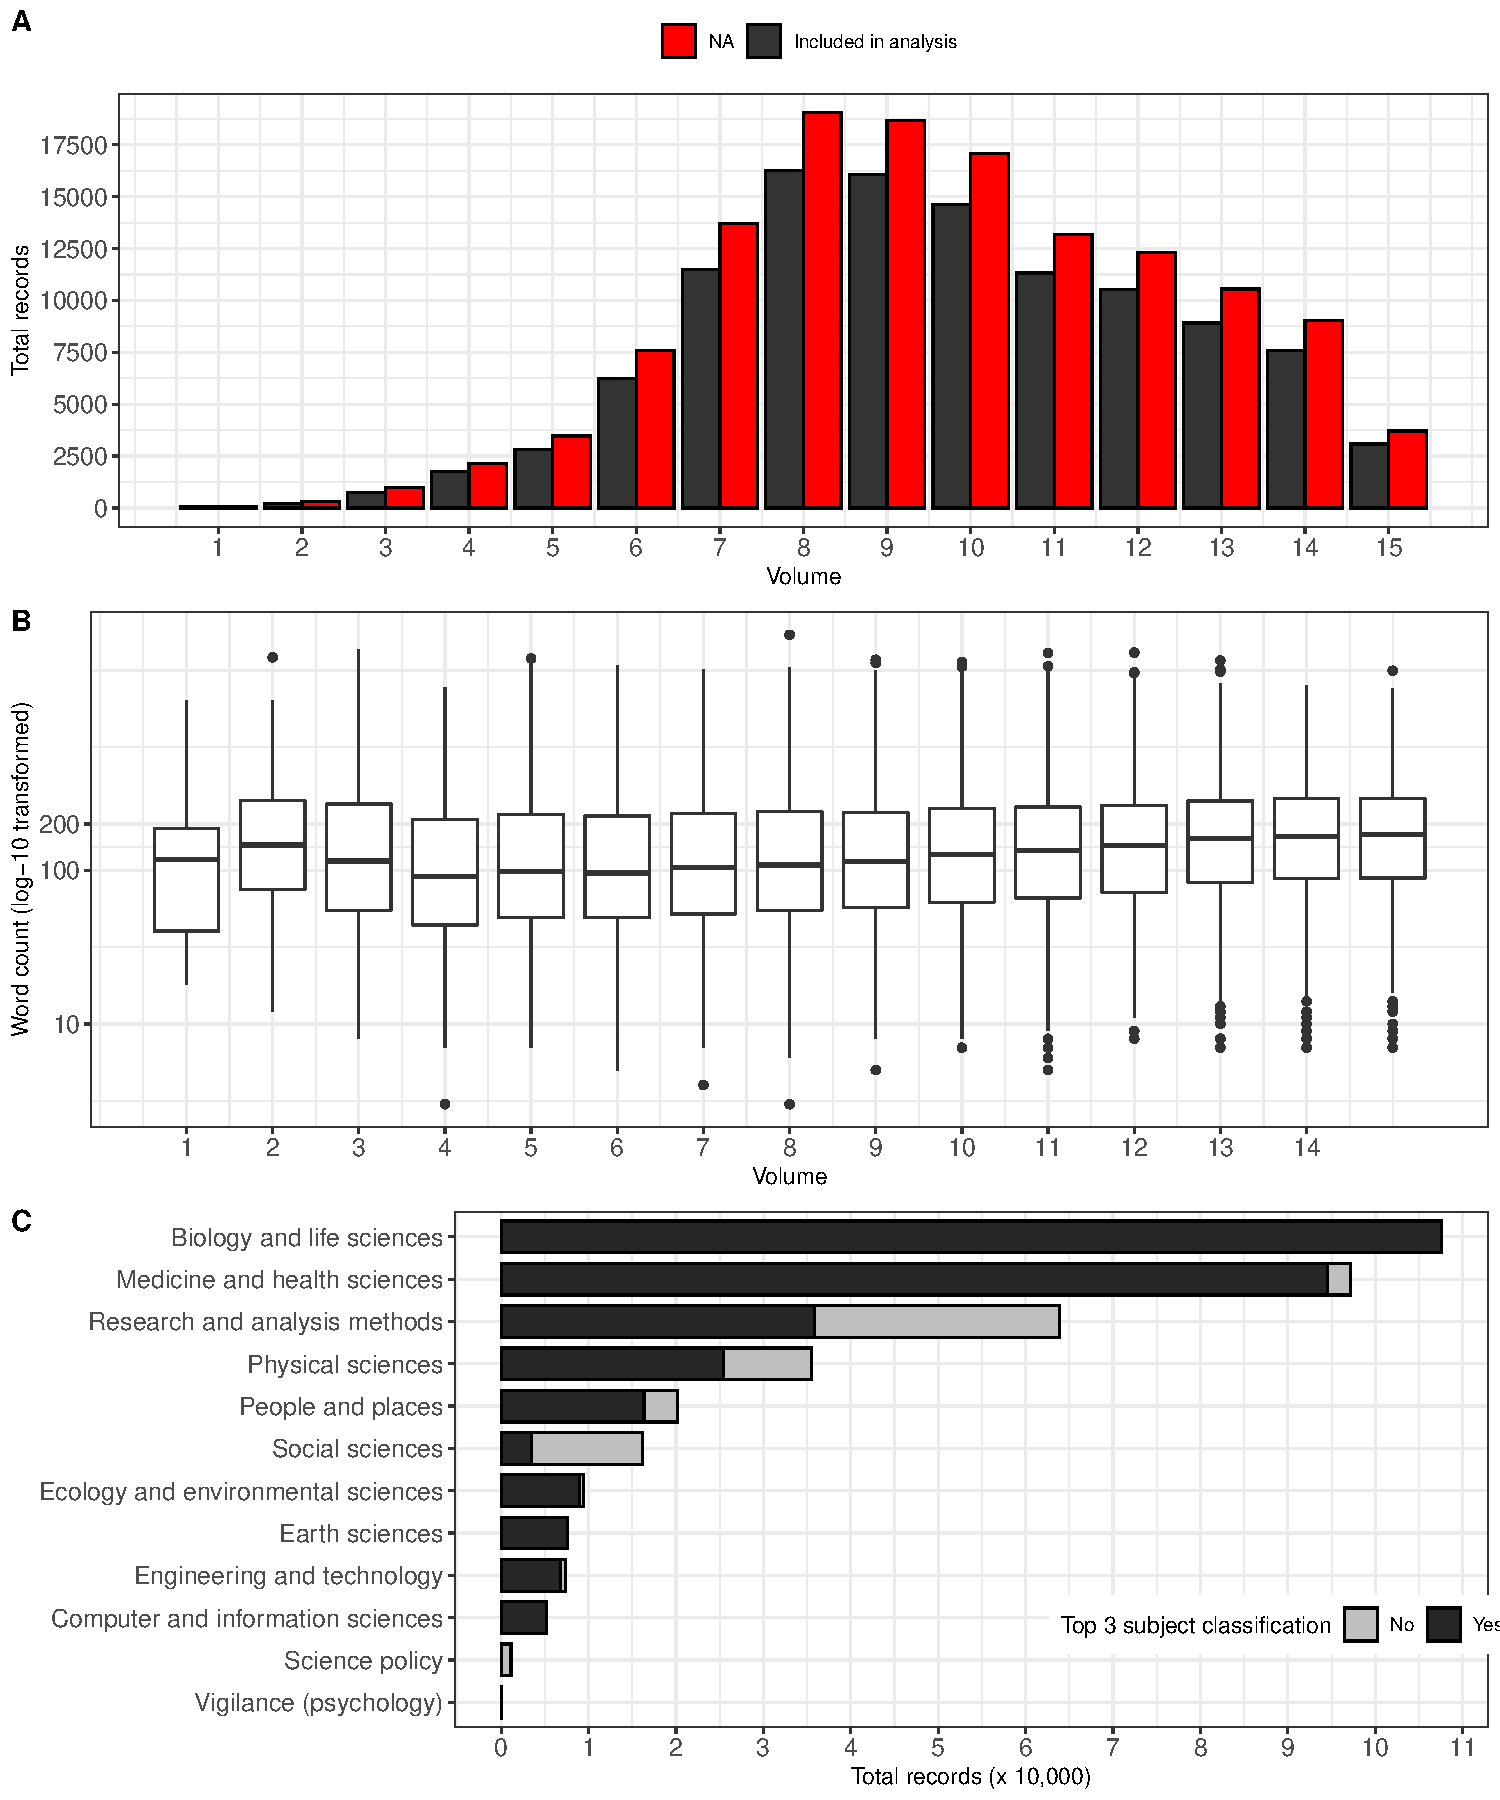
\includegraphics{draft_manuscript_files/figure-latex/unnamed-chunk-3-1.pdf}
\caption{\label{fig:plos-n}Search results by PLOS ONE volume (1st row);
word count per statistical methods section included in analysis (n =
111,731; 2nd row); subject classifications assigned to full-text records
included in analysis (3rd row)}
\end{figure}

API searches returned 131847 unique records, of which 111731 (85\%)
included a statistical methods section based on our search criteria.
Search results varied by journal volume (Figure 1A). The total number of
API search results peaked at volumes 8 (n = 19045) and 9 (n = 19045),
corresponding to years 2013 and 2014. This trend aligned with the total
number of papers published in PLOS ONE over the same timeframe. The
percentage of records that included a statistical methods section by
volume based on our proposed matching criteria varied between 64\%
(volume 2) and 86\% (volume 9).

The median length of statistical methods sections after text cleaning
was 127 per DOI (IQR: 61 to 254) (Figure 1B).

Across all records included in analysis, all included Biology and life
sciences (n = 107584), Earth sciences (n = 7605) and/or Computer and
information sciences (n = 5190) within their top 3 subject
classifications (Figure 1C).

{[}Figure here or as supplementary - 5 topic solution{]}

Results of topic modelling assuming five clusters showed clear
separation between statistical software, hypothesis testing and linear
modelling (Figure). The largest cluster, representing 48\% of all
included studies (Topic 2, n = 53,491).

Two topics (26\% of study sample) were dominated by terms related
statistical software, notably Prism/GraphPad (Topic 3, n = 10,940) and
SPSS (Topic 5, n = 18,029). Remaining topics focussed on hypothesis
testing (Topic, n = 12,531) and analysis of variance/multiple
comparisons (Topic 4, n = 16,740)

Top matches (Topic 3)

\begin{itemize}
\tightlist
\item
  10.1371/journal.pone.0043519: All statistical analyses were performed
  using GraphPad Prism (GraphPad Software Inc., San Diego, CA).
\item
  10.1371/journal.pone.0045453: GraphPad Prism (Graphpad Software, San
  Diego, CA) was used for all analyses.
\item
  10.1371/journal.pone.0170640: All statistical analysis of the data was
  performed using GraphPad Prism software (GraphPad Prism Software Inc.,
  La Jolla, Ca).
\item
  10.1371/journal.pone.0036750: All statistical analysis was performed
  using Graphpad Prism software.
\item
  10.1371/journal.pone.0058148: All statistical analysis was performed
  using the Graphpad Prism software.
\end{itemize}

Top matches (Topic 5) * 10.1371/journal.pone.0120046: Statistical
analysis was performed using the SPSS version 18.0 (SPSS Inc., Chicago,
IL, USA). Mann-Whitney test was used for the analysis of continuous
variables. Chi-square test, Fisher's exact test or one-way ANOVA test
was employed for the analysis of categorical variables. P \textless{}
0.05 was considered statistically significant.

\begin{itemize}
\item
  10.1371/journal.pone.0204950: Statistical analyses were performed
  using SPSS version 20.0 for Windows (SPSS Inc., Chicago, IL).
  Categorical and continuous variables were evaluated with the
  non-parametric chi-square test, the Kruskal-Wallis test, and the
  Mann-Whitney U test. All statistical tests were two-sided, and a p
  value \textless0.05 was considered statistically significant.
\item
  10.1371/journal.pone.0062685: SPSS version 21.0 for Windows (SPSS,
  Inc., Chicago, IL, USA) was used for statistical analysis. Categorical
  variables were analyzed by a chi-square test or Fisher's exact test.
  Continuous variables were analyzed by independent t-test or
  Mann-Whitney test. Logistic regression analysis was performed to
  evaluate the effects of independent variables on clinical outcomes. A
  p-value of \textless0.05 by the two-tailed test was considered
  statistically significant.
\item
  10.1371/journal.pone.0133783: Data are expressed as means ± SD or
  medians (with interquartile ranges). Statistical analyses were
  performed using SPSS software version 19.0 (SPSS, Inc., Chicago, IL,
  USA). Statistical significance for intergroup differences was assessed
  by the χ2 test or Fisher's exact test for categorical variables, and
  by the Student's t-test, or Mann--Whitney U test for continuous
  variables. Correlations between variables were tested with Spearman's
  correlation analysis. A P-value \textless0.05 was considered
  significant for all tests.
\item
  10.1371/journal.pone.0098797: Univariate analysis was performed using
  Mann--Whitney U-tests for continuous variables and Pearson's
  chi-square or Fisher's exact tests for categorical variables.
  Statistical significance was set at a P-value \textless0.05. SPSS
  statistical software version 19 (SPSS, Chicago, IL, USA) was used to
  perform the statistical analyses.
\end{itemize}

{[}Figure here or as supplementary - 10 topic solution{]}

\hypertarget{anzctr}{%
\subsection{ANZCTR}\label{anzctr}}

We downloaded 28,008 studies. The numbers of excluded studies are shown
in Figure\textasciitilde X. Of the 12,700 included studies, 9,523 had a
statistic section which is 75\% (95\% CI 74\% to 76\%).

We examined if four study characteristics were associated with a missing
statistics section. The odds ratios and 95\% credible intervals are in
Table\textasciitilde X. Observational studies were less likely to have a
missing methods section compared with interventional studies. Missing
sections became less likely over time. Studies with more funders and a
larger target sample size were less likely to have a missing methods
section.

Variable \& Odds ratio \& 95\% CI Study type = Observational \& 0.78 \&
0.69, 0.89 Date (per year) \& 0.90 \& 0.88, 0.91 Number of funders \&
0.80 \& 0.74, 0.86 Target sample size (per doubling) \& 0.90 \& 0.88,
0.92

Some of the non-missing statistics sections were only one word,
including ``ANOVA'', ``t-test'', ``SPSS'' and even ``SSPS''. The median
length of the section was 129 words with an inter-quartile range of 71
to 219 words.

\begin{itemize}
\tightlist
\item
  Final sample size
\end{itemize}

\hypertarget{discussion}{%
\section{Discussion}\label{discussion}}

Many researchers are using lazy practice by copying a standard
``boilerplate'' statistical methods section, likely cut-and-pasting from
other researchers or projects. This is a strong sign of the ritualistic
practice of statistics where researchers go through the motions rather
than using conscientious practice (Stark and Saltelli
\protect\hyperlink{ref-Stark2018}{2018}). This is concerning because
using the wrong statistical methods can reduce the potential of study,
or worse, invalidate the entire study. Poor statistical practice is a
key driver of the ongoing reproducibility crisis in science (Ioannidis
et al. \protect\hyperlink{ref-Ioannidis2014}{2014}).

The first line in many statistical analysis sections in \emph{PLOS ONE}
was the software used and some entire sections in ANZCTR only stated the
software, implying that the software is the most important detail. As
Doug Altman said, ``Many people think that all you need to do statistics
is a computer and appropriate software'' (Altman
\protect\hyperlink{ref-Altman1994}{1994}). This is not the case, and
whilst it is important for researchers to mention the software and
version used for reproducibility purposes, it is a minor detail compared
with detailing what methods were used and why.

Despite the extensive array of statistical tests available, many authors
are reporting the same few methods.

One reason these inadequate sections get published is that most journals
do not use statistical reviewers, despite empirical evidence showing
they improve manuscript quality (Hardwicke and Goodman
\protect\hyperlink{ref-Hardwicke2020}{2020}).

\hypertarget{limitations}{%
\subsection{Limitations}\label{limitations}}

We did not check whether papers used the correct methods, and for some
simple studies a `boilerplate' statistical methods section would be
fine.

We examined papers where there was a statistics section, and we missed
papers that used statistical analysis but did not include a statistical
analysis section. Reiterate outcomes of random sample checking here.

We only examined one journal and one trial registry and hence our
results may not be generalisable to all journals or registries,
especially those that consistently use a statistical reviewer.

We searched the full text of \emph{PLOS ONE} papers but not the
supporting information which may contain statistical methods sections
for some papers. The search terms we used to find statistical methods
appeared in the supporting information titles for xxx papers (x\%). We
did not include the supporting information because it is less structured
than the paper and could be in PDF or Word format.

\hypertarget{references}{%
\section*{References}\label{references}}
\addcontentsline{toc}{section}{References}

\hypertarget{refs}{}
\leavevmode\hypertarget{ref-Allison2016}{}%
Allison, David B., Andrew W. Brown, Brandon J. George, and Kathryn A.
Kaiser. 2016. ``Reproducibility: A Tragedy of Errors.'' \emph{Nature}
530 (7588): 27--29. \url{https://doi.org/10.1038/530027a}.

\leavevmode\hypertarget{ref-Altman1994}{}%
Altman, D G. 1994. ``The Scandal of Poor Medical Research.'' \emph{BMJ}
308 (6924): 283--84. \url{https://doi.org/10.1136/bmj.308.6924.283}.

\leavevmode\hypertarget{ref-Altman2016}{}%
Altman, Douglas G, and Iveta Simera. 2016. ``A History of the Evolution
of Guidelines for Reporting Medical Research: The Long Road to the
EQUATOR Network.'' \emph{Journal of the Royal Society of Medicine} 109
(2): 67--77. \url{https://doi.org/10.1177/0141076815625599}.

\leavevmode\hypertarget{ref-ANZCTR}{}%
anzctr. 2019. ``ANZCTR Data Field Definitions V25.''
\url{https://www.anzctr.org.au/docs/ANZCTR\%20Data\%20field\%20explanation.pdf}.

\leavevmode\hypertarget{ref-rplos}{}%
Chamberlain, Scott, Carl Boettiger, and Karthik Ram. 2020. \emph{Rplos:
Interface to the Search API for 'PLoS' Journals}.
\url{https://CRAN.R-project.org/package=rplos}.

\leavevmode\hypertarget{ref-Ernst2017}{}%
Ernst, Anja F., and Casper J. Albers. 2017. ``Regression Assumptions in
Clinical Psychology Research Practicea Systematic Review of Common
Misconceptions.'' \emph{PeerJ} 5: e3323.
\url{https://doi.org/10.7717/peerj.3323}.

\leavevmode\hypertarget{ref-Goodman2008}{}%
Goodman, Steven. 2008. ``A Dirty Dozen: Twelve P-Value Misconceptions.''
\emph{Seminars in Hematology} 45 (3): 135--40.
\url{https://doi.org/10.1053/j.seminhematol.2008.04.003}.

\leavevmode\hypertarget{ref-Goodman1998}{}%
Goodman, Steven N., Douglas G. Altman, and Stephen L. George. 1998.
``Statistical Reviewing Policies of Medical Journals.'' \emph{Journal of
General Internal Medicine} 13 (11): 753--56.
\url{https://doi.org/10.1046/j.1525-1497.1998.00227.x}.

\leavevmode\hypertarget{ref-Hardwicke2020}{}%
Hardwicke, Tom E, and Steve Goodman. 2020. ``How Often Do Leading
Biomedical Journalsuse Statistical Experts to Evaluate Statistical
Methods? The Results of a Survey.'' MetaArXiv.
\url{https://doi.org/10.31222/osf.io/z27u4}.

\leavevmode\hypertarget{ref-ICMJE2019}{}%
ICJME. 2019. ``Recommendations for the Conduct, Reporting, Editing, and
Publication of Scholarly Work in Medical Journals.''
\url{http://www.icmje.org/icmje-recommendations.pdf}.

\leavevmode\hypertarget{ref-Ioannidis2014}{}%
Ioannidis, John P A, Sander Greenland, Mark A Hlatky, Muin J Khoury,
Malcolm R Macleod, David Moher, Kenneth F Schulz, and Robert Tibshirani.
2014. ``Increasing Value and Reducing Waste in Research Design, Conduct,
and Analysis.'' \emph{The Lancet} 383 (9912): 166--75.
\url{https://doi.org/10.1016/s0140-6736(13)62227-8}.

\leavevmode\hypertarget{ref-King2019}{}%
King, Kevin M., Michael D. Pullmann, Aaron R. Lyon, Shannon Dorsey, and
Cara C. Lewis. 2019. ``Using Implementation Science to Close the Gap
Between the Optimal and Typical Practice of Quantitative Methods in
Clinical Science.'' \emph{Journal of Abnormal Psychology} 128 (6):
547--62. \url{https://doi.org/10.1037/abn0000417}.

\leavevmode\hypertarget{ref-Leek2017}{}%
Leek, Jeff, Blakeley B. McShane, Andrew Gelman, David Colquhoun, Michèle
B. Nuijten, and Steven N. Goodman. 2017. ``Five Ways to Fix
Statistics.'' \emph{Nature} 551 (7682): 557--59.
\url{https://doi.org/10.1038/d41586-017-07522-z}.

\leavevmode\hypertarget{ref-textclean}{}%
Rinker, Tyler W. 2018. \emph{textclean: Text Cleaning Tools}. Buffalo,
New York. \url{https://github.com/trinker/textclean}.

\leavevmode\hypertarget{ref-Stark2018}{}%
Stark, Philip B., and Andrea Saltelli. 2018. ``Cargo-Cult Statistics and
Scientific Crisis.'' \emph{Significance} 15 (4): 40--43.
\url{https://doi.org/10.1111/j.1740-9713.2018.01174.x}.

\leavevmode\hypertarget{ref-Zhou2018}{}%
Zhou, Yuanyuan, and Susan Skidmore. 2018. ``A Reassessment of ANOVA
Reporting Practices: A Review of Three APA Journals.'' \emph{Journal of
Methods and Measurement in the Social Sciences} 8 (1): 3--19.
\url{https://doi.org/10.2458/v8i1.22019}.

\end{document}
